% Bit layouts of every numeric format in the study.
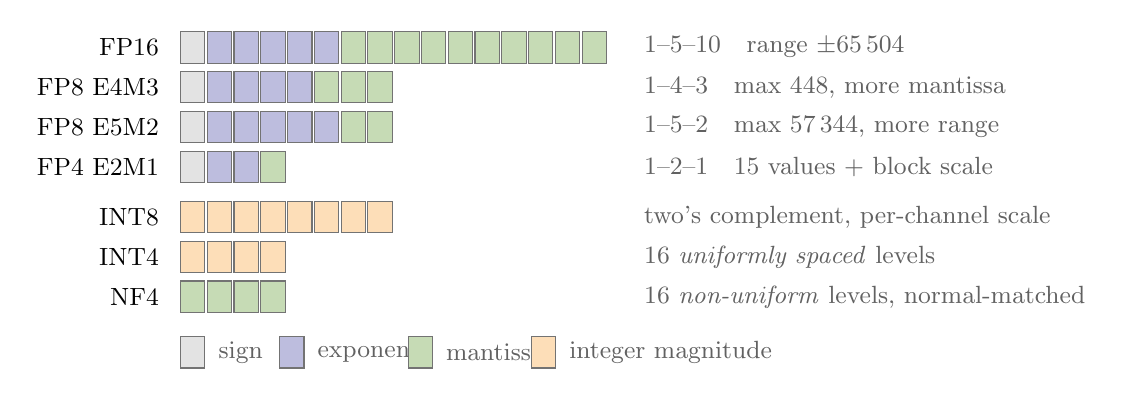
\begin{tikzpicture}[
  x=3.4mm, y=4.4mm, font=\small,
  sgn/.style={draw=black!55, fill=gray!22, minimum width=3.1mm, minimum height=4mm, inner sep=0pt},
  exp/.style={draw=black!55, fill=NavyBlue!26, minimum width=3.1mm, minimum height=4mm, inner sep=0pt},
  man/.style={draw=black!55, fill=OliveGreen!24, minimum width=3.1mm, minimum height=4mm, inner sep=0pt},
  int/.style={draw=black!55, fill=BurntOrange!24, minimum width=3.1mm, minimum height=4mm, inner sep=0pt},
  lbl/.style={anchor=east, font=\small},
  note/.style={anchor=west, font=\small, text=black!62},
]
\def\row#1#2#3#4#5{%
  \node[lbl] at (-0.4,#1) {#2};
  \foreach \i in {1,...,#3} { \node[sgn] at (\i-0.5,#1) {}; }
  \pgfmathsetmacro{\a}{#3}
  \foreach \i in {1,...,#4} { \node[exp] at (\a+\i-0.5,#1) {}; }
  \pgfmathsetmacro{\b}{#3+#4}
  \foreach \i in {1,...,#5} { \node[man] at (\b+\i-0.5,#1) {}; }
}
% label            sign exp mantissa
\row{0}{FP16}{1}{5}{10}
\node[note] at (17,0) {1--5--10\quad range $\pm$65\,504};
\row{-1.15}{FP8 E4M3}{1}{4}{3}
\node[note] at (17,-1.15) {1--4--3\quad max 448, more mantissa};
\row{-2.3}{FP8 E5M2}{1}{5}{2}
\node[note] at (17,-2.3) {1--5--2\quad max 57\,344, more range};
\row{-3.45}{FP4 E2M1}{1}{2}{1}
\node[note] at (17,-3.45) {1--2--1\quad 15 values + block scale};

% integers
\node[lbl] at (-0.4,-4.9) {INT8};
\foreach \i in {1,...,8} { \node[int] at (\i-0.5,-4.9) {}; }
\node[note] at (17,-4.9) {two's complement, per-channel scale};
\node[lbl] at (-0.4,-6.05) {INT4};
\foreach \i in {1,...,4} { \node[int] at (\i-0.5,-6.05) {}; }
\node[note] at (17,-6.05) {16 \emph{uniformly spaced} levels};

% NF4 codebook
\node[lbl] at (-0.4,-7.2) {NF4};
\foreach \i in {1,...,4} { \node[man] at (\i-0.5,-7.2) {}; }
\node[note] at (17,-7.2) {16 \emph{non-uniform} levels, normal-matched};

% legend
\node[sgn] at (0.5,-8.8) {}; \node[note] at (1.1,-8.8) {sign};
\node[exp] at (4.2,-8.8) {}; \node[note] at (4.8,-8.8) {exponent};
\node[man] at (9.0,-8.8) {}; \node[note] at (9.6,-8.8) {mantissa};
\node[int] at (13.6,-8.8) {}; \node[note] at (14.2,-8.8) {integer magnitude};
\end{tikzpicture}
